% Compile twice with pdflatex from this directory.
\documentclass[aspectratio=169,11pt]{beamer}
\usetheme{Madrid}
\usecolortheme{seahorse}
\usepackage[T1]{fontenc}
\usepackage[utf8]{inputenc}
\usepackage{lmodern}
\usepackage{tikz}
\usetikzlibrary{arrows.meta}
\definecolor{teal}{HTML}{367775}
\definecolor{ink}{HTML}{183B3C}
\setbeamercolor{structure}{fg=teal}
\setbeamercolor{palette primary}{fg=white,bg=teal}
\setbeamercolor{palette secondary}{fg=white,bg=ink}
\setbeamercolor{palette tertiary}{fg=white,bg=ink}
\setbeamercolor{title}{fg=white,bg=ink}
\setbeamercolor{frametitle}{fg=white,bg=ink}
\setbeamercolor{block title}{fg=white,bg=teal}
\setbeamercolor{block body}{fg=ink,bg=teal!4}
\setbeamertemplate{navigation symbols}{}
\setbeamertemplate{footline}{\leavevmode\hbox{%
\begin{beamercolorbox}[wd=.8\paperwidth,ht=2.5ex,dp=1ex,leftskip=1em]{palette tertiary}\scriptsize TrashUQ\end{beamercolorbox}%
\begin{beamercolorbox}[wd=.2\paperwidth,ht=2.5ex,dp=1ex,rightskip=1em plus1fil]{palette primary}\hfill\insertframenumber\,/\,\inserttotalframenumber\end{beamercolorbox}}}
\title[TrashUQ]{TrashUQ}
\subtitle{Federated learning for intelligent waste monitoring}
\author[TrashUQ team]{Aleix Bertran Andreu \and Pol Llinàs Vaquer\\[0.3em] Bru Pallàs Vargués \and Aleix Rosinach Olivart}
\date{}
\hypersetup{pdftitle={TrashUQ},pdfauthor={Aleix Bertran Andreu, Pol Llinàs Vaquer, Bru Pallàs Vargués, Aleix Rosinach Olivart}}
\begin{document}

\begin{frame}
\titlepage
\end{frame}

\begin{frame}{Federated learning with less communication}
\setbeamerfont{block title}{size=\small}
\begin{columns}[T,onlytextwidth]
\begin{column}{.49\textwidth}
\begin{block}{How the Arduinos learn together}
\centering
\vspace{.1cm}
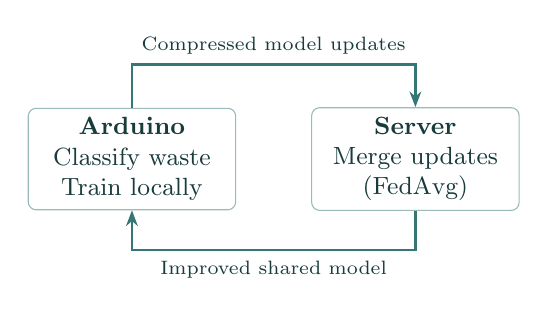
\begin{tikzpicture}[every node/.style={text=ink,align=center,font=\small},
 box/.style={draw=teal!50,fill=white,rounded corners=1mm,text width=2.4cm,minimum height=1.15cm},
 arr/.style={-{Stealth[length=2mm]},teal,line width=.8pt}]
\node[box] (device) at (0,0) {\textbf{Arduino}\\Classify waste\\Train locally};
\node[box] (server) at (3.6,0) {\textbf{Server}\\Merge updates\\(FedAvg)};
\draw[arr] (device.north)--++(0,.55)-|node[pos=.25,above,font=\scriptsize]{Compressed model updates} (server.north);
\draw[arr] (server.south)--++(0,-.5)-|node[pos=.25,below,font=\scriptsize]{Improved shared model} (device.south);
\end{tikzpicture}
\par\smallskip
\small Images stay on the Arduino.
\par\smallskip
\end{block}
\end{column}
\begin{column}{.47\textwidth}
\begin{block}{Which compression worked best?}
\small We compared stochastic rounding (SR)\\and Top-k sparsification.
\par\smallskip
\centering
{\scriptsize Total communication (MB)}\par\smallskip
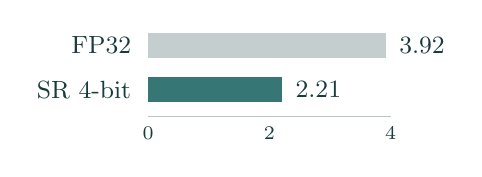
\begin{tikzpicture}[x=.77cm,y=.75cm,every node/.style={font=\small,text=ink}]
\node[anchor=east] at (-.12,1.1){FP32};
\node[anchor=east] at (-.12,.35){SR 4-bit};
\fill[ink!25] (0,.89) rectangle (3.922,1.31);
\fill[teal] (0,.14) rectangle (2.210,.56);
\node[anchor=west] at (3.98,1.1){3.92};
\node[anchor=west] at (2.27,.35){2.21};
\draw[ink!30] (0,-.1)--(4,-.1);
\foreach \v in {0,2,4}{\node[anchor=north,font=\scriptsize] at (\v,-.12){\v};}
\end{tikzpicture}
\par\smallskip
\end{block}
\end{column}
\end{columns}
\smallskip
\begin{beamercolorbox}[sep=.1cm,center,rounded=true]{block title}
\textbf{SR 4-bit: 44\% less communication, with no accuracy loss}
\end{beamercolorbox}
\smallskip
\end{frame}

\begin{frame}{Thank you}
\begin{columns}[c,onlytextwidth]
\begin{column}{.58\textwidth}
{\LARGE\bfseries\color{ink}Questions?\par}
\bigskip
{\large Thanks for listening.\par}
\medskip
{\color{teal}Scan to explore the project.}
\end{column}
\begin{column}{.4\textwidth}
\centering
\resizebox{4.6cm}{!}{% Exact QR modules from poster/main.tex: https://trashuq.vercel.app

\begin{tikzpicture}[x=0.105cm,y=0.105cm]
\path[fill=white] (-4,4) rectangle (29,-29);
\fill[black] (0,0) rectangle ++(1,-1);
\fill[black] (1,0) rectangle ++(1,-1);
\fill[black] (2,0) rectangle ++(1,-1);
\fill[black] (3,0) rectangle ++(1,-1);
\fill[black] (4,0) rectangle ++(1,-1);
\fill[black] (5,0) rectangle ++(1,-1);
\fill[black] (6,0) rectangle ++(1,-1);
\fill[black] (8,0) rectangle ++(1,-1);
\fill[black] (9,0) rectangle ++(1,-1);
\fill[black] (16,0) rectangle ++(1,-1);
\fill[black] (18,0) rectangle ++(1,-1);
\fill[black] (19,0) rectangle ++(1,-1);
\fill[black] (20,0) rectangle ++(1,-1);
\fill[black] (21,0) rectangle ++(1,-1);
\fill[black] (22,0) rectangle ++(1,-1);
\fill[black] (23,0) rectangle ++(1,-1);
\fill[black] (24,0) rectangle ++(1,-1);
\fill[black] (0,-1) rectangle ++(1,-1);
\fill[black] (6,-1) rectangle ++(1,-1);
\fill[black] (18,-1) rectangle ++(1,-1);
\fill[black] (24,-1) rectangle ++(1,-1);
\fill[black] (0,-2) rectangle ++(1,-1);
\fill[black] (2,-2) rectangle ++(1,-1);
\fill[black] (3,-2) rectangle ++(1,-1);
\fill[black] (4,-2) rectangle ++(1,-1);
\fill[black] (6,-2) rectangle ++(1,-1);
\fill[black] (8,-2) rectangle ++(1,-1);
\fill[black] (11,-2) rectangle ++(1,-1);
\fill[black] (12,-2) rectangle ++(1,-1);
\fill[black] (13,-2) rectangle ++(1,-1);
\fill[black] (14,-2) rectangle ++(1,-1);
\fill[black] (15,-2) rectangle ++(1,-1);
\fill[black] (18,-2) rectangle ++(1,-1);
\fill[black] (20,-2) rectangle ++(1,-1);
\fill[black] (21,-2) rectangle ++(1,-1);
\fill[black] (22,-2) rectangle ++(1,-1);
\fill[black] (24,-2) rectangle ++(1,-1);
\fill[black] (0,-3) rectangle ++(1,-1);
\fill[black] (2,-3) rectangle ++(1,-1);
\fill[black] (3,-3) rectangle ++(1,-1);
\fill[black] (4,-3) rectangle ++(1,-1);
\fill[black] (6,-3) rectangle ++(1,-1);
\fill[black] (8,-3) rectangle ++(1,-1);
\fill[black] (9,-3) rectangle ++(1,-1);
\fill[black] (11,-3) rectangle ++(1,-1);
\fill[black] (13,-3) rectangle ++(1,-1);
\fill[black] (14,-3) rectangle ++(1,-1);
\fill[black] (15,-3) rectangle ++(1,-1);
\fill[black] (16,-3) rectangle ++(1,-1);
\fill[black] (18,-3) rectangle ++(1,-1);
\fill[black] (20,-3) rectangle ++(1,-1);
\fill[black] (21,-3) rectangle ++(1,-1);
\fill[black] (22,-3) rectangle ++(1,-1);
\fill[black] (24,-3) rectangle ++(1,-1);
\fill[black] (0,-4) rectangle ++(1,-1);
\fill[black] (2,-4) rectangle ++(1,-1);
\fill[black] (3,-4) rectangle ++(1,-1);
\fill[black] (4,-4) rectangle ++(1,-1);
\fill[black] (6,-4) rectangle ++(1,-1);
\fill[black] (8,-4) rectangle ++(1,-1);
\fill[black] (9,-4) rectangle ++(1,-1);
\fill[black] (10,-4) rectangle ++(1,-1);
\fill[black] (11,-4) rectangle ++(1,-1);
\fill[black] (15,-4) rectangle ++(1,-1);
\fill[black] (16,-4) rectangle ++(1,-1);
\fill[black] (18,-4) rectangle ++(1,-1);
\fill[black] (20,-4) rectangle ++(1,-1);
\fill[black] (21,-4) rectangle ++(1,-1);
\fill[black] (22,-4) rectangle ++(1,-1);
\fill[black] (24,-4) rectangle ++(1,-1);
\fill[black] (0,-5) rectangle ++(1,-1);
\fill[black] (6,-5) rectangle ++(1,-1);
\fill[black] (9,-5) rectangle ++(1,-1);
\fill[black] (12,-5) rectangle ++(1,-1);
\fill[black] (16,-5) rectangle ++(1,-1);
\fill[black] (18,-5) rectangle ++(1,-1);
\fill[black] (24,-5) rectangle ++(1,-1);
\fill[black] (0,-6) rectangle ++(1,-1);
\fill[black] (1,-6) rectangle ++(1,-1);
\fill[black] (2,-6) rectangle ++(1,-1);
\fill[black] (3,-6) rectangle ++(1,-1);
\fill[black] (4,-6) rectangle ++(1,-1);
\fill[black] (5,-6) rectangle ++(1,-1);
\fill[black] (6,-6) rectangle ++(1,-1);
\fill[black] (8,-6) rectangle ++(1,-1);
\fill[black] (10,-6) rectangle ++(1,-1);
\fill[black] (12,-6) rectangle ++(1,-1);
\fill[black] (14,-6) rectangle ++(1,-1);
\fill[black] (16,-6) rectangle ++(1,-1);
\fill[black] (18,-6) rectangle ++(1,-1);
\fill[black] (19,-6) rectangle ++(1,-1);
\fill[black] (20,-6) rectangle ++(1,-1);
\fill[black] (21,-6) rectangle ++(1,-1);
\fill[black] (22,-6) rectangle ++(1,-1);
\fill[black] (23,-6) rectangle ++(1,-1);
\fill[black] (24,-6) rectangle ++(1,-1);
\fill[black] (9,-7) rectangle ++(1,-1);
\fill[black] (11,-7) rectangle ++(1,-1);
\fill[black] (14,-7) rectangle ++(1,-1);
\fill[black] (15,-7) rectangle ++(1,-1);
\fill[black] (16,-7) rectangle ++(1,-1);
\fill[black] (0,-8) rectangle ++(1,-1);
\fill[black] (1,-8) rectangle ++(1,-1);
\fill[black] (2,-8) rectangle ++(1,-1);
\fill[black] (3,-8) rectangle ++(1,-1);
\fill[black] (6,-8) rectangle ++(1,-1);
\fill[black] (8,-8) rectangle ++(1,-1);
\fill[black] (14,-8) rectangle ++(1,-1);
\fill[black] (15,-8) rectangle ++(1,-1);
\fill[black] (16,-8) rectangle ++(1,-1);
\fill[black] (17,-8) rectangle ++(1,-1);
\fill[black] (20,-8) rectangle ++(1,-1);
\fill[black] (21,-8) rectangle ++(1,-1);
\fill[black] (22,-8) rectangle ++(1,-1);
\fill[black] (24,-8) rectangle ++(1,-1);
\fill[black] (0,-9) rectangle ++(1,-1);
\fill[black] (1,-9) rectangle ++(1,-1);
\fill[black] (7,-9) rectangle ++(1,-1);
\fill[black] (9,-9) rectangle ++(1,-1);
\fill[black] (17,-9) rectangle ++(1,-1);
\fill[black] (19,-9) rectangle ++(1,-1);
\fill[black] (23,-9) rectangle ++(1,-1);
\fill[black] (1,-10) rectangle ++(1,-1);
\fill[black] (2,-10) rectangle ++(1,-1);
\fill[black] (4,-10) rectangle ++(1,-1);
\fill[black] (6,-10) rectangle ++(1,-1);
\fill[black] (7,-10) rectangle ++(1,-1);
\fill[black] (13,-10) rectangle ++(1,-1);
\fill[black] (14,-10) rectangle ++(1,-1);
\fill[black] (16,-10) rectangle ++(1,-1);
\fill[black] (17,-10) rectangle ++(1,-1);
\fill[black] (20,-10) rectangle ++(1,-1);
\fill[black] (0,-11) rectangle ++(1,-1);
\fill[black] (3,-11) rectangle ++(1,-1);
\fill[black] (4,-11) rectangle ++(1,-1);
\fill[black] (8,-11) rectangle ++(1,-1);
\fill[black] (11,-11) rectangle ++(1,-1);
\fill[black] (12,-11) rectangle ++(1,-1);
\fill[black] (13,-11) rectangle ++(1,-1);
\fill[black] (14,-11) rectangle ++(1,-1);
\fill[black] (16,-11) rectangle ++(1,-1);
\fill[black] (18,-11) rectangle ++(1,-1);
\fill[black] (21,-11) rectangle ++(1,-1);
\fill[black] (22,-11) rectangle ++(1,-1);
\fill[black] (0,-12) rectangle ++(1,-1);
\fill[black] (1,-12) rectangle ++(1,-1);
\fill[black] (3,-12) rectangle ++(1,-1);
\fill[black] (6,-12) rectangle ++(1,-1);
\fill[black] (8,-12) rectangle ++(1,-1);
\fill[black] (9,-12) rectangle ++(1,-1);
\fill[black] (11,-12) rectangle ++(1,-1);
\fill[black] (12,-12) rectangle ++(1,-1);
\fill[black] (13,-12) rectangle ++(1,-1);
\fill[black] (14,-12) rectangle ++(1,-1);
\fill[black] (15,-12) rectangle ++(1,-1);
\fill[black] (16,-12) rectangle ++(1,-1);
\fill[black] (17,-12) rectangle ++(1,-1);
\fill[black] (18,-12) rectangle ++(1,-1);
\fill[black] (19,-12) rectangle ++(1,-1);
\fill[black] (20,-12) rectangle ++(1,-1);
\fill[black] (22,-12) rectangle ++(1,-1);
\fill[black] (23,-12) rectangle ++(1,-1);
\fill[black] (24,-12) rectangle ++(1,-1);
\fill[black] (1,-13) rectangle ++(1,-1);
\fill[black] (2,-13) rectangle ++(1,-1);
\fill[black] (3,-13) rectangle ++(1,-1);
\fill[black] (4,-13) rectangle ++(1,-1);
\fill[black] (5,-13) rectangle ++(1,-1);
\fill[black] (7,-13) rectangle ++(1,-1);
\fill[black] (8,-13) rectangle ++(1,-1);
\fill[black] (9,-13) rectangle ++(1,-1);
\fill[black] (10,-13) rectangle ++(1,-1);
\fill[black] (11,-13) rectangle ++(1,-1);
\fill[black] (14,-13) rectangle ++(1,-1);
\fill[black] (15,-13) rectangle ++(1,-1);
\fill[black] (16,-13) rectangle ++(1,-1);
\fill[black] (17,-13) rectangle ++(1,-1);
\fill[black] (18,-13) rectangle ++(1,-1);
\fill[black] (19,-13) rectangle ++(1,-1);
\fill[black] (20,-13) rectangle ++(1,-1);
\fill[black] (24,-13) rectangle ++(1,-1);
\fill[black] (1,-14) rectangle ++(1,-1);
\fill[black] (4,-14) rectangle ++(1,-1);
\fill[black] (5,-14) rectangle ++(1,-1);
\fill[black] (6,-14) rectangle ++(1,-1);
\fill[black] (8,-14) rectangle ++(1,-1);
\fill[black] (9,-14) rectangle ++(1,-1);
\fill[black] (10,-14) rectangle ++(1,-1);
\fill[black] (13,-14) rectangle ++(1,-1);
\fill[black] (14,-14) rectangle ++(1,-1);
\fill[black] (20,-14) rectangle ++(1,-1);
\fill[black] (22,-14) rectangle ++(1,-1);
\fill[black] (23,-14) rectangle ++(1,-1);
\fill[black] (0,-15) rectangle ++(1,-1);
\fill[black] (2,-15) rectangle ++(1,-1);
\fill[black] (3,-15) rectangle ++(1,-1);
\fill[black] (4,-15) rectangle ++(1,-1);
\fill[black] (9,-15) rectangle ++(1,-1);
\fill[black] (10,-15) rectangle ++(1,-1);
\fill[black] (12,-15) rectangle ++(1,-1);
\fill[black] (14,-15) rectangle ++(1,-1);
\fill[black] (15,-15) rectangle ++(1,-1);
\fill[black] (16,-15) rectangle ++(1,-1);
\fill[black] (17,-15) rectangle ++(1,-1);
\fill[black] (18,-15) rectangle ++(1,-1);
\fill[black] (19,-15) rectangle ++(1,-1);
\fill[black] (20,-15) rectangle ++(1,-1);
\fill[black] (24,-15) rectangle ++(1,-1);
\fill[black] (2,-16) rectangle ++(1,-1);
\fill[black] (3,-16) rectangle ++(1,-1);
\fill[black] (4,-16) rectangle ++(1,-1);
\fill[black] (5,-16) rectangle ++(1,-1);
\fill[black] (6,-16) rectangle ++(1,-1);
\fill[black] (7,-16) rectangle ++(1,-1);
\fill[black] (8,-16) rectangle ++(1,-1);
\fill[black] (11,-16) rectangle ++(1,-1);
\fill[black] (12,-16) rectangle ++(1,-1);
\fill[black] (13,-16) rectangle ++(1,-1);
\fill[black] (16,-16) rectangle ++(1,-1);
\fill[black] (17,-16) rectangle ++(1,-1);
\fill[black] (18,-16) rectangle ++(1,-1);
\fill[black] (19,-16) rectangle ++(1,-1);
\fill[black] (20,-16) rectangle ++(1,-1);
\fill[black] (21,-16) rectangle ++(1,-1);
\fill[black] (22,-16) rectangle ++(1,-1);
\fill[black] (23,-16) rectangle ++(1,-1);
\fill[black] (24,-16) rectangle ++(1,-1);
\fill[black] (8,-17) rectangle ++(1,-1);
\fill[black] (11,-17) rectangle ++(1,-1);
\fill[black] (12,-17) rectangle ++(1,-1);
\fill[black] (15,-17) rectangle ++(1,-1);
\fill[black] (16,-17) rectangle ++(1,-1);
\fill[black] (20,-17) rectangle ++(1,-1);
\fill[black] (22,-17) rectangle ++(1,-1);
\fill[black] (24,-17) rectangle ++(1,-1);
\fill[black] (0,-18) rectangle ++(1,-1);
\fill[black] (1,-18) rectangle ++(1,-1);
\fill[black] (2,-18) rectangle ++(1,-1);
\fill[black] (3,-18) rectangle ++(1,-1);
\fill[black] (4,-18) rectangle ++(1,-1);
\fill[black] (5,-18) rectangle ++(1,-1);
\fill[black] (6,-18) rectangle ++(1,-1);
\fill[black] (9,-18) rectangle ++(1,-1);
\fill[black] (10,-18) rectangle ++(1,-1);
\fill[black] (12,-18) rectangle ++(1,-1);
\fill[black] (14,-18) rectangle ++(1,-1);
\fill[black] (16,-18) rectangle ++(1,-1);
\fill[black] (18,-18) rectangle ++(1,-1);
\fill[black] (20,-18) rectangle ++(1,-1);
\fill[black] (22,-18) rectangle ++(1,-1);
\fill[black] (23,-18) rectangle ++(1,-1);
\fill[black] (24,-18) rectangle ++(1,-1);
\fill[black] (0,-19) rectangle ++(1,-1);
\fill[black] (6,-19) rectangle ++(1,-1);
\fill[black] (11,-19) rectangle ++(1,-1);
\fill[black] (14,-19) rectangle ++(1,-1);
\fill[black] (15,-19) rectangle ++(1,-1);
\fill[black] (16,-19) rectangle ++(1,-1);
\fill[black] (20,-19) rectangle ++(1,-1);
\fill[black] (23,-19) rectangle ++(1,-1);
\fill[black] (24,-19) rectangle ++(1,-1);
\fill[black] (0,-20) rectangle ++(1,-1);
\fill[black] (2,-20) rectangle ++(1,-1);
\fill[black] (3,-20) rectangle ++(1,-1);
\fill[black] (4,-20) rectangle ++(1,-1);
\fill[black] (6,-20) rectangle ++(1,-1);
\fill[black] (9,-20) rectangle ++(1,-1);
\fill[black] (12,-20) rectangle ++(1,-1);
\fill[black] (16,-20) rectangle ++(1,-1);
\fill[black] (17,-20) rectangle ++(1,-1);
\fill[black] (18,-20) rectangle ++(1,-1);
\fill[black] (19,-20) rectangle ++(1,-1);
\fill[black] (20,-20) rectangle ++(1,-1);
\fill[black] (21,-20) rectangle ++(1,-1);
\fill[black] (24,-20) rectangle ++(1,-1);
\fill[black] (0,-21) rectangle ++(1,-1);
\fill[black] (2,-21) rectangle ++(1,-1);
\fill[black] (3,-21) rectangle ++(1,-1);
\fill[black] (4,-21) rectangle ++(1,-1);
\fill[black] (6,-21) rectangle ++(1,-1);
\fill[black] (8,-21) rectangle ++(1,-1);
\fill[black] (10,-21) rectangle ++(1,-1);
\fill[black] (11,-21) rectangle ++(1,-1);
\fill[black] (13,-21) rectangle ++(1,-1);
\fill[black] (15,-21) rectangle ++(1,-1);
\fill[black] (17,-21) rectangle ++(1,-1);
\fill[black] (18,-21) rectangle ++(1,-1);
\fill[black] (20,-21) rectangle ++(1,-1);
\fill[black] (21,-21) rectangle ++(1,-1);
\fill[black] (22,-21) rectangle ++(1,-1);
\fill[black] (23,-21) rectangle ++(1,-1);
\fill[black] (24,-21) rectangle ++(1,-1);
\fill[black] (0,-22) rectangle ++(1,-1);
\fill[black] (2,-22) rectangle ++(1,-1);
\fill[black] (3,-22) rectangle ++(1,-1);
\fill[black] (4,-22) rectangle ++(1,-1);
\fill[black] (6,-22) rectangle ++(1,-1);
\fill[black] (8,-22) rectangle ++(1,-1);
\fill[black] (9,-22) rectangle ++(1,-1);
\fill[black] (11,-22) rectangle ++(1,-1);
\fill[black] (12,-22) rectangle ++(1,-1);
\fill[black] (13,-22) rectangle ++(1,-1);
\fill[black] (16,-22) rectangle ++(1,-1);
\fill[black] (18,-22) rectangle ++(1,-1);
\fill[black] (20,-22) rectangle ++(1,-1);
\fill[black] (22,-22) rectangle ++(1,-1);
\fill[black] (23,-22) rectangle ++(1,-1);
\fill[black] (0,-23) rectangle ++(1,-1);
\fill[black] (6,-23) rectangle ++(1,-1);
\fill[black] (8,-23) rectangle ++(1,-1);
\fill[black] (9,-23) rectangle ++(1,-1);
\fill[black] (10,-23) rectangle ++(1,-1);
\fill[black] (13,-23) rectangle ++(1,-1);
\fill[black] (20,-23) rectangle ++(1,-1);
\fill[black] (22,-23) rectangle ++(1,-1);
\fill[black] (0,-24) rectangle ++(1,-1);
\fill[black] (1,-24) rectangle ++(1,-1);
\fill[black] (2,-24) rectangle ++(1,-1);
\fill[black] (3,-24) rectangle ++(1,-1);
\fill[black] (4,-24) rectangle ++(1,-1);
\fill[black] (5,-24) rectangle ++(1,-1);
\fill[black] (6,-24) rectangle ++(1,-1);
\fill[black] (8,-24) rectangle ++(1,-1);
\fill[black] (9,-24) rectangle ++(1,-1);
\fill[black] (12,-24) rectangle ++(1,-1);
\fill[black] (13,-24) rectangle ++(1,-1);
\fill[black] (14,-24) rectangle ++(1,-1);
\fill[black] (17,-24) rectangle ++(1,-1);
\fill[black] (19,-24) rectangle ++(1,-1);
\fill[black] (20,-24) rectangle ++(1,-1);
\fill[black] (21,-24) rectangle ++(1,-1);
\fill[black] (22,-24) rectangle ++(1,-1);
\fill[black] (23,-24) rectangle ++(1,-1);
\fill[black] (24,-24) rectangle ++(1,-1);
\end{tikzpicture}
}
\end{column}
\end{columns}
\end{frame}
\end{document}
